%%%%%%%%%%%%%%%%%%%%%%%%%%%%%%%%%%%%%%%%%
% Beamer Presentation
% LaTeX Template
% Version 1.0 (10/11/12)
%
% This template has been downloaded from:
% http://www.LaTeXTemplates.com
%
% License:
% CC BY-NC-SA 3.0 (http://creativecommons.org/licenses/by-nc-sa/3.0/)
%
%%%%%%%%%%%%%%%%%%%%%%%%%%%%%%%%%%%%%%%%%

%----------------------------------------------------------------------------------------
%	PACKAGES AND THEMES
%----------------------------------------------------------------------------------------

\documentclass{beamer}

\mode<presentation> {

% The Beamer class comes with a number of default slide themes
% which change the colors and layouts of slides. Below this is a list
% of all the themes, uncomment each in turn to see what they look like.

%\usetheme{default}
%\usetheme{AnnArbor}
%\usetheme{Antibes}
%\usetheme{Bergen}
%\usetheme{Berkeley}
\usetheme{Berlin}
%\usetheme{Boadilla}
%\usetheme{CambridgeUS}
%\usetheme{Copenhagen}
%\usetheme{Darmstadt}
%\usetheme{Dresden}
%\usetheme{Frankfurt}
%\usetheme{Goettingen}
%\usetheme{Hannover}
%\usetheme{Ilmenau}
%\usetheme{JuanLesPins}
%\usetheme{Luebeck}
%\usetheme{Madrid}
%\usetheme{Malmoe}
%\usetheme{Marburg}
%\usetheme{Montpellier}
%\usetheme{PaloAlto}
%\usetheme{Pittsburgh}
%\usetheme{Rochester}
%\usetheme{Singapore}
%\usetheme{Szeged}
%\usetheme{Warsaw}

% As well as themes, the Beamer class has a number of color themes
% for any slide theme. Uncomment each of these in turn to see how it
% changes the colors of your current slide theme.

%\usecolortheme{albatross}
%\usecolortheme{beaver}
%\usecolortheme{beetle}
%\usecolortheme{crane}
%\usecolortheme{dolphin}
%\usecolortheme{dove}
%\usecolortheme{fly}
%\usecolortheme{lily}
%\usecolortheme{orchid}
%\usecolortheme{rose}
%\usecolortheme{seagull}
%\usecolortheme{seahorse}
%\usecolortheme{whale}
%\usecolortheme{wolverine}

%\setbeamertemplate{footline} % To remove the footer line in all slides uncomment this line
%\setbeamertemplate{footline}[page number] % To replace the footer line in all slides with a simple slide count uncomment this line

%\setbeamertemplate{navigation symbols}{} % To remove the navigation symbols from the bottom of all slides uncomment this line
}

\usepackage{graphicx} % Allows including images
\usepackage{booktabs} % Allows the use of \toprule, \midrule and \bottomrule in tables
%\usepackage[brazilian]{babel}
\usepackage[utf8]{inputenc}
\usepackage{listings}
\usepackage{amsmath}
\usepackage{amsfonts}
\usepackage{pdfpages}
\usepackage{textpos}

\graphicspath{ {img/} }

%----------------------------------------------------------------------------------------
%	TITLE PAGE
%----------------------------------------------------------------------------------------

\title[Generating Acrostics via Paraphrasing and Heuristic Search]{Generating Acrostics via Paraphrasing and Heuristic Search} % The short title appears at the bottom of every slide, the full title is only on the title page

\author[Bruno, Fernando, Jürgen, William]{Bruno Soares Fillmann\\
Fernando Bombardelli da Silva\\
Jürgen Bauer\\
William Bombardelli da Silva
} % Your name
\institute[TU Berlin] % Your institution as it will appear on the bottom of every slide, may be shorthand to save space
{
Technische Universität Berlin \\ % Your institution for the title page
Datenbanksysteme und Informationsmanagement \\
DBPRO – Database Projects (WS 2014/2015) \\
\medskip
%\textit{fbdasilva@inf.ufrgs.br} % Your email address
}
\date{01.12.2014} % Date, can be changed to a custom date

\begin{document}

\begin{frame}
\titlepage % Print the title page as the first slide
\end{frame}

\begin{frame}
\frametitle{Organisation} % Table of contents slide, comment this block out to remove it
\tableofcontents % Throughout your presentation, if you choose to use \section{} and \subsection{} commands, these will automatically be printed on this slide as an overview of your presentation
\end{frame}

%----------------------------------------------------------------------------------------
%	PRESENTATION SLIDES
%----------------------------------------------------------------------------------------

%------------------------------------------------
\section{Overview} % Sections can be created in order to organize your presentation into discrete blocks, all sections and subsections are automatically printed in the table of contents as an overview of the talk
%------------------------------------------------

%\subsection{Subsection Example} % A subsection can be created just before a set of slides with a common theme to further break down your presentation into chunks

\begin{frame}
\frametitle{Overview}
\begin{itemize}
\item \textbf{The problem:} Given a text T and an acrostic X, find a paraphased version of T that encodes X in the first letters of each line.
\item \textbf{Main goal of the project:} Implement the paper for the German language.
\item \textbf{Main idea of the algorithm:}
	\begin{itemize}
	\item Modeled as a search problem in a tree.
	\item The vertices are states (texts) and the edges are operations over states.
	\item Artificial inteligence is applied for the search strategy (A* Algorithm).
	\end{itemize}
\end{itemize}
\end{frame}

\begin{frame}
\frametitle{Classes Diagram}
\begin{figure}
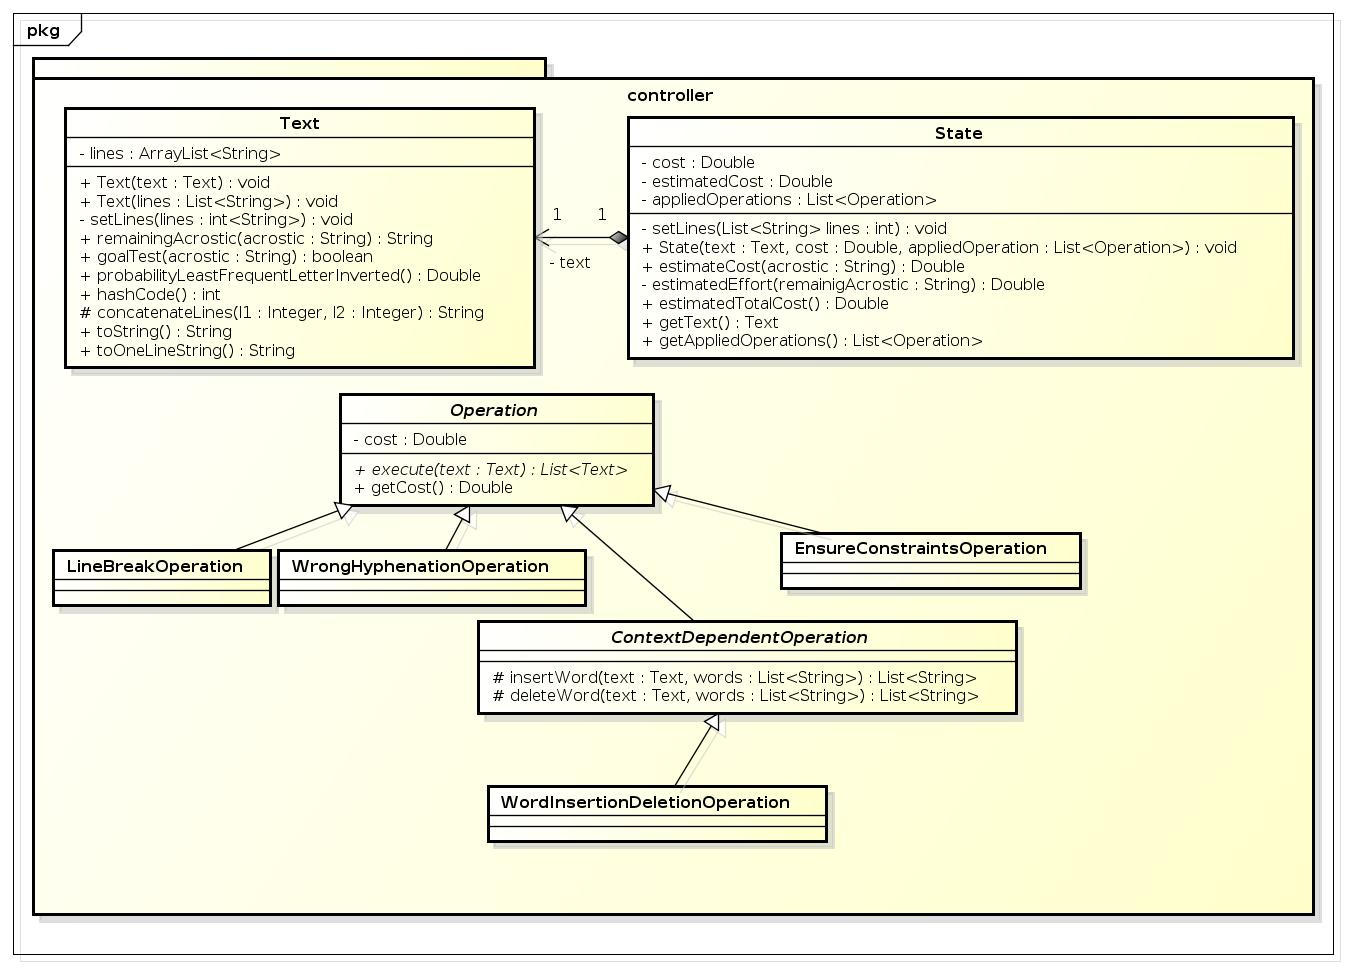
\includegraphics[scale=0.2]{Controller}
\end{figure}
\end{frame}

\begin{frame}
\frametitle{Activity Diagram and Search Strategy}
\begin{figure}
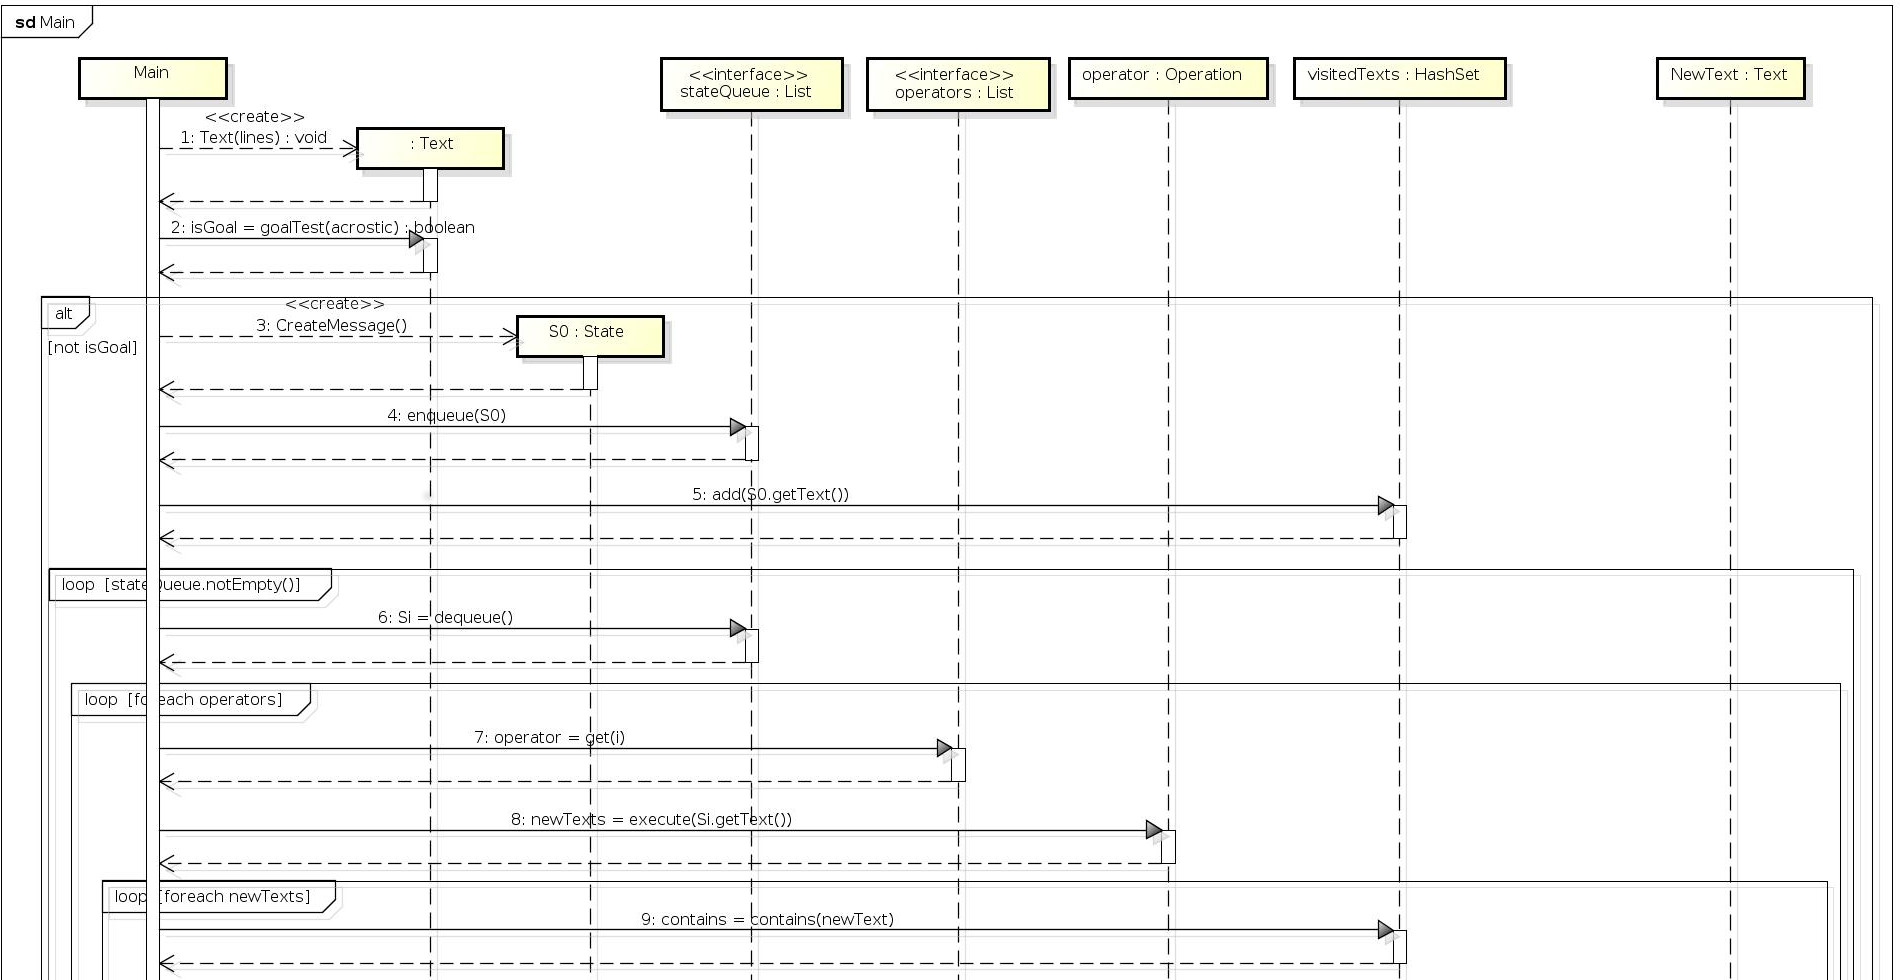
\includegraphics[scale=0.16]{Main_1}
\end{figure}
\end{frame}

\begin{frame}
\frametitle{Activity Diagram and Search Strategy}
\begin{figure}
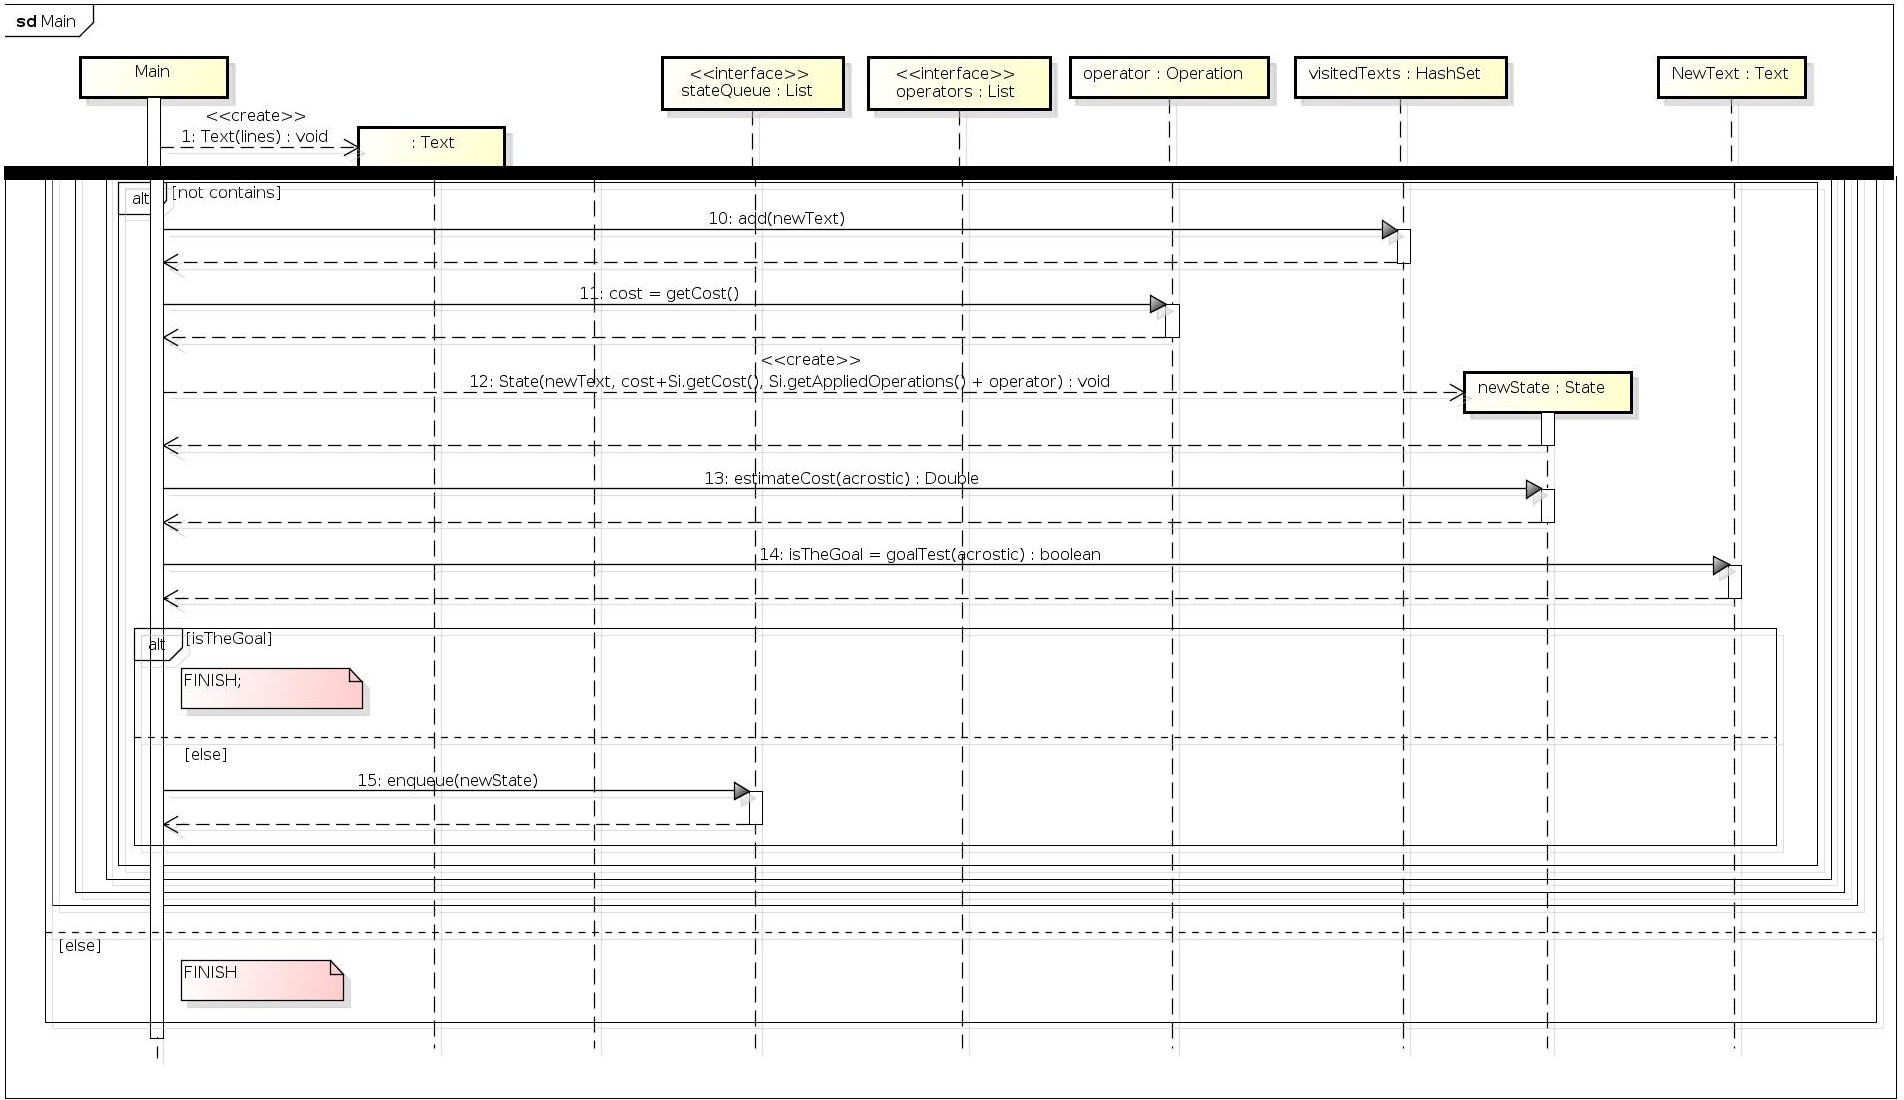
\includegraphics[scale=0.16]{Main_2}
\end{figure}
\end{frame}

%------------------------------------------------
\section{Implemented Operations}
%------------------------------------------------

\begin{frame}
\frametitle{Line Break}


\begin{itemize}
\item Constraints on line length $l_{min}=50$ and $l_{max}=70.$



\item Two cases: 



\begin{itemize}
\item After a word when line length falls in the\\
 $[l_{min},l_{max}]$-window.
\item After a full stop. (i.e., paragraph break)
\end{itemize}


\item Succeeding line break, lines have to be aligned.

\item A greedy word wrap algorithm is applied. 

\item Avoid words of length $>20$ in the start text.
\end{itemize}

\end{frame}



\begin{frame}
\frametitle{Line Break}

%\begin{textblock}{200}(0,0)
%\leavevmode
%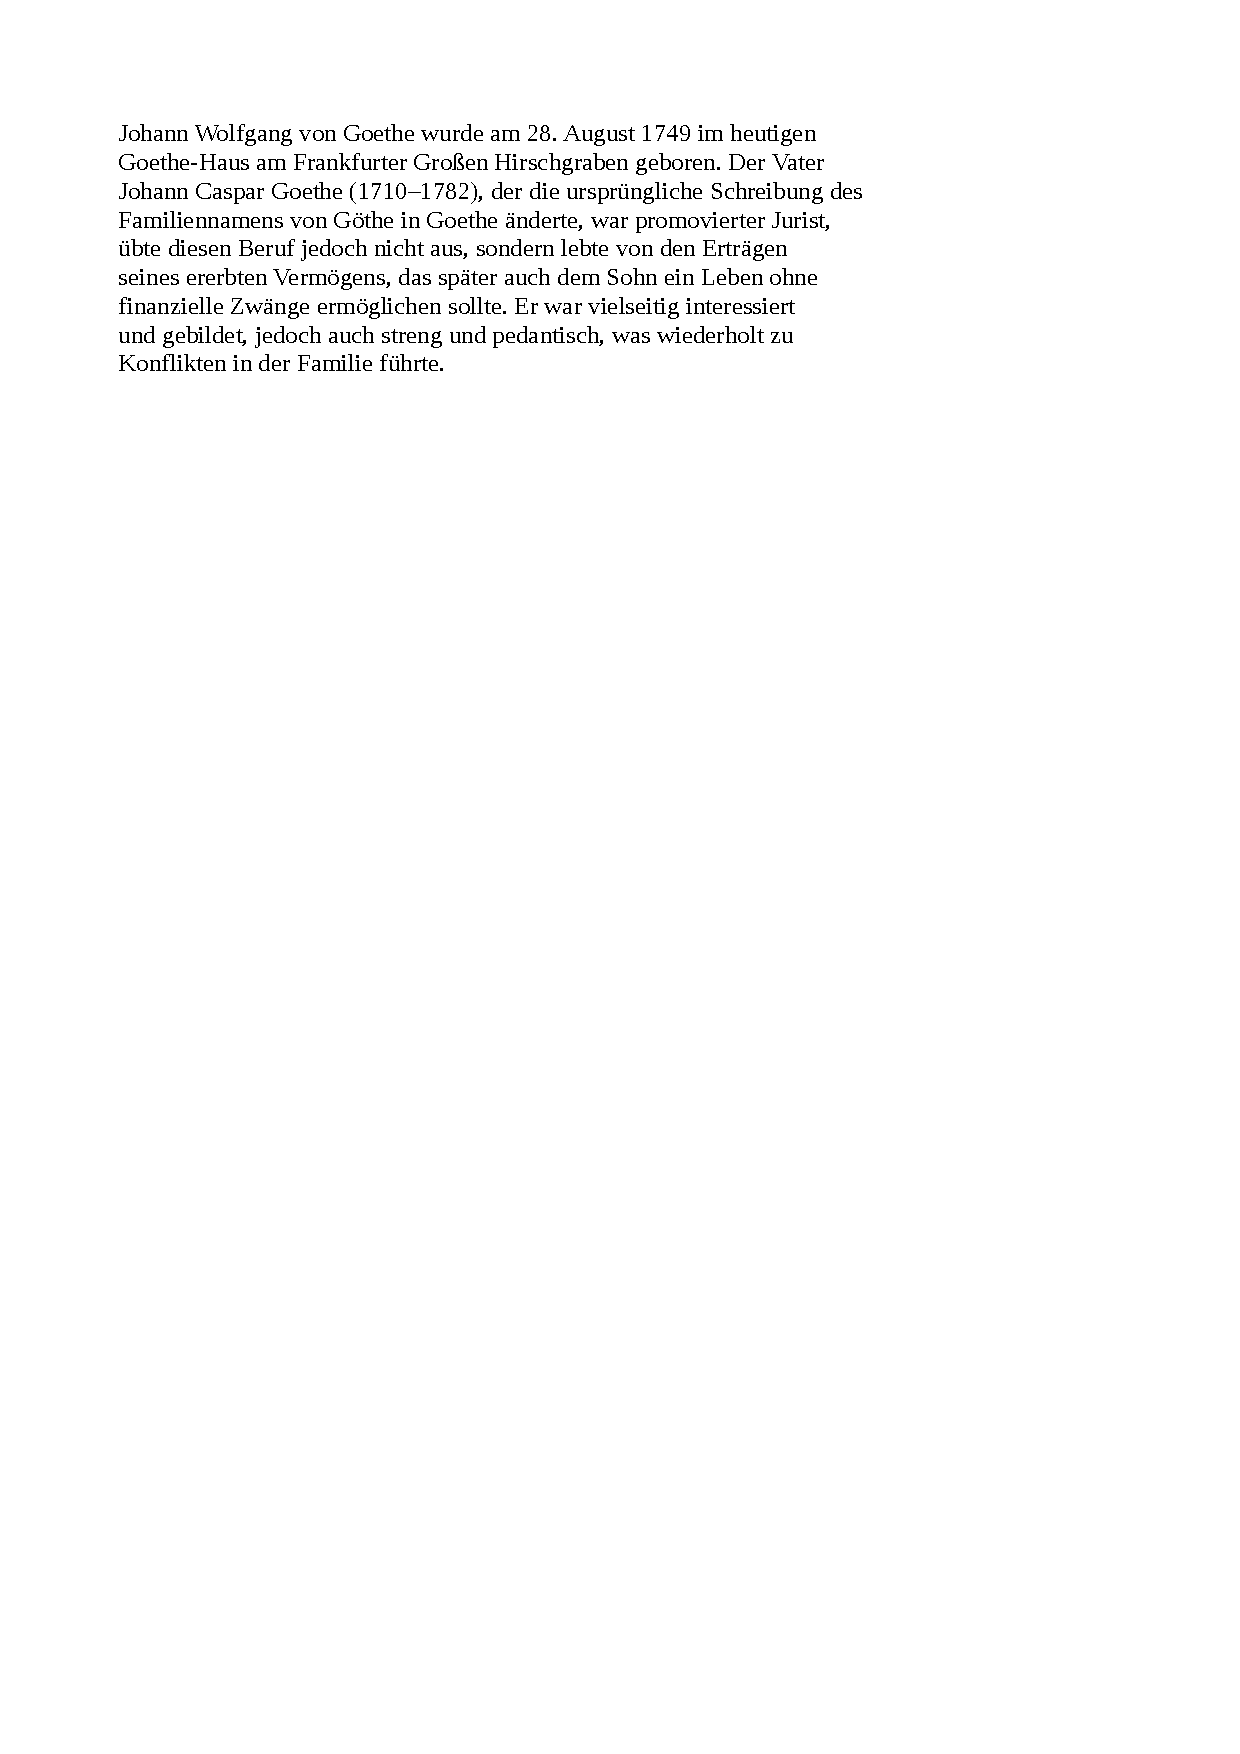
\includegraphics[scale=0.5]{Goethe.pdf}

%\put(0,50){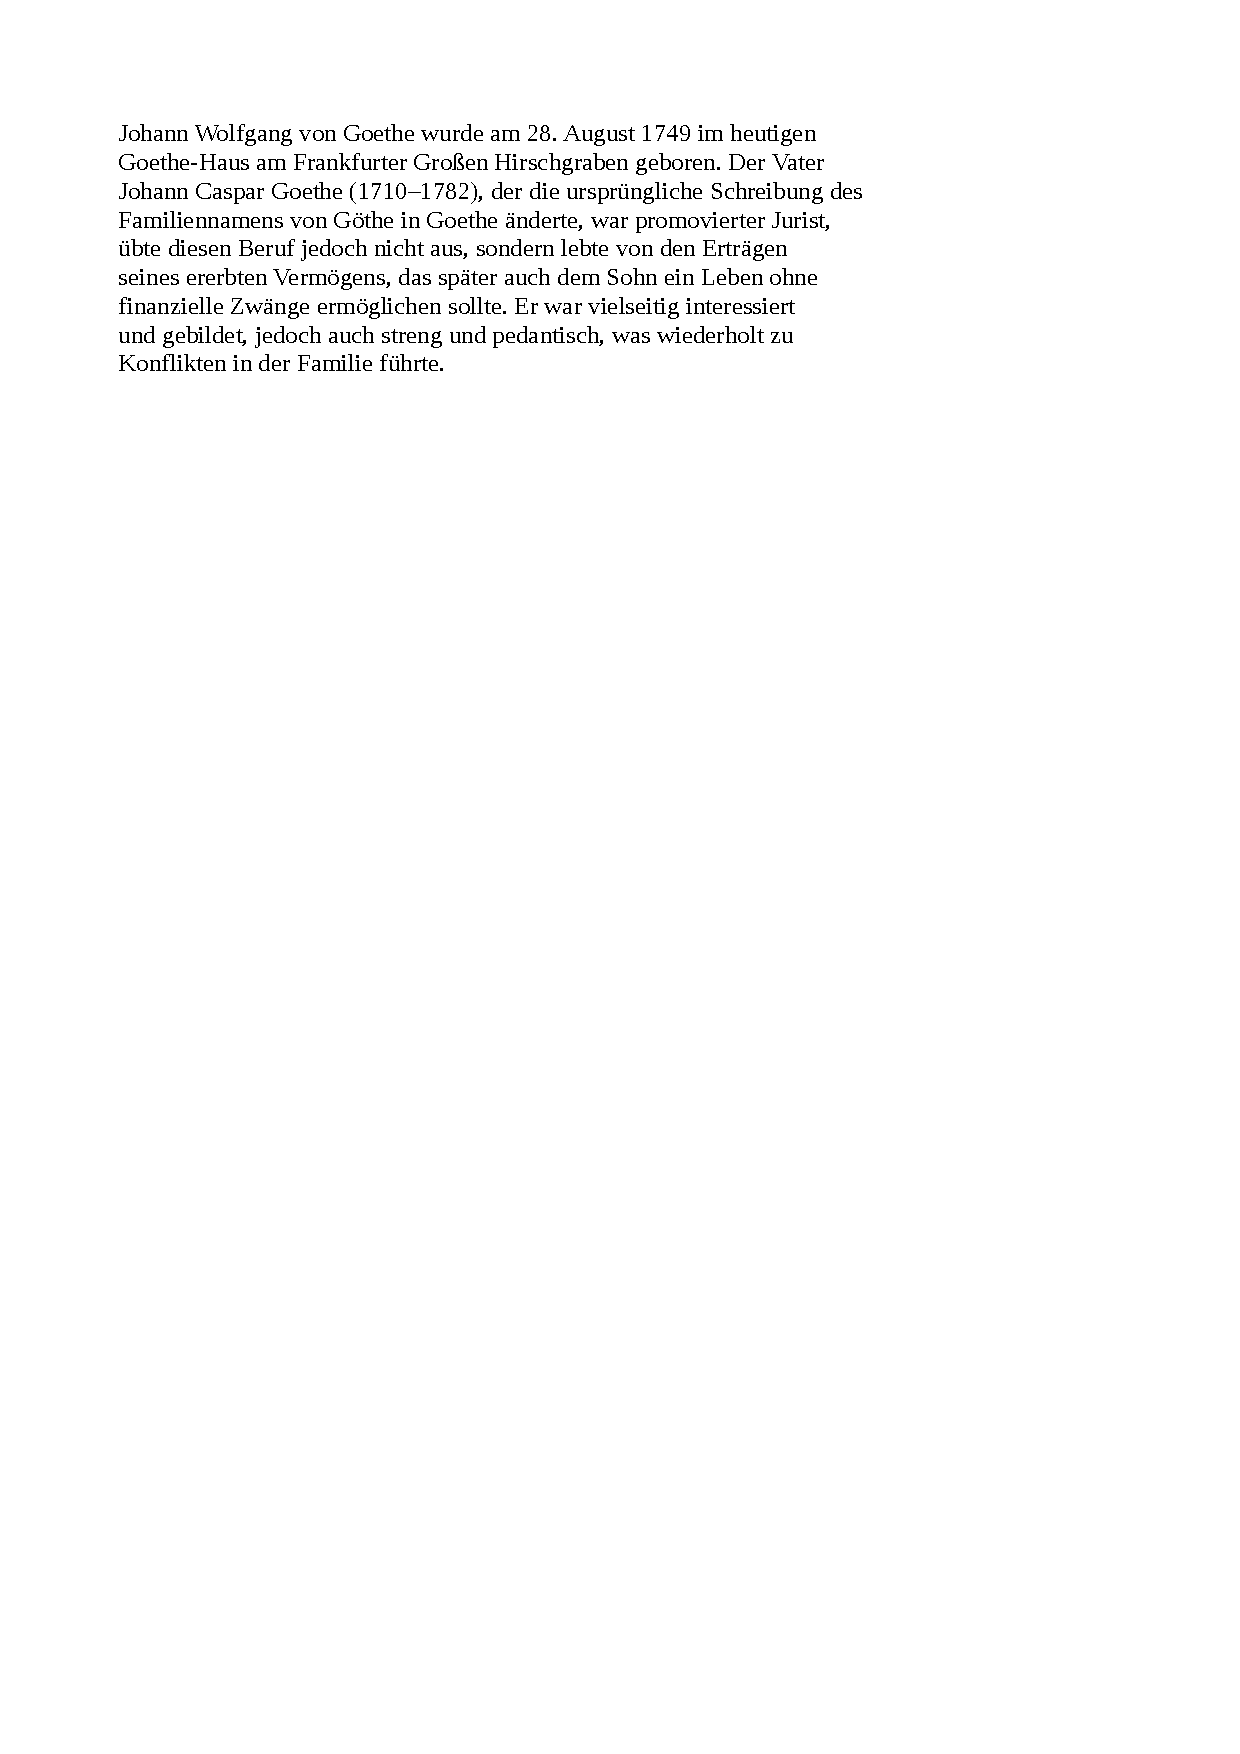
\includegraphics[scale=0.5]{Goethe.pdf}}
%\end{textblock}

\begin{itemize}
\item \textbf{Example:}
\item 18 linebreaks,
\item No full stop after 28!
\item Third often applied operator on a solution path
\item Fastest operator
%\item Hier steht ein längerer Text mit Foto
%\end{itemize}

\end{itemize}

\begin{picture}(300,400)
\put(-10,-165){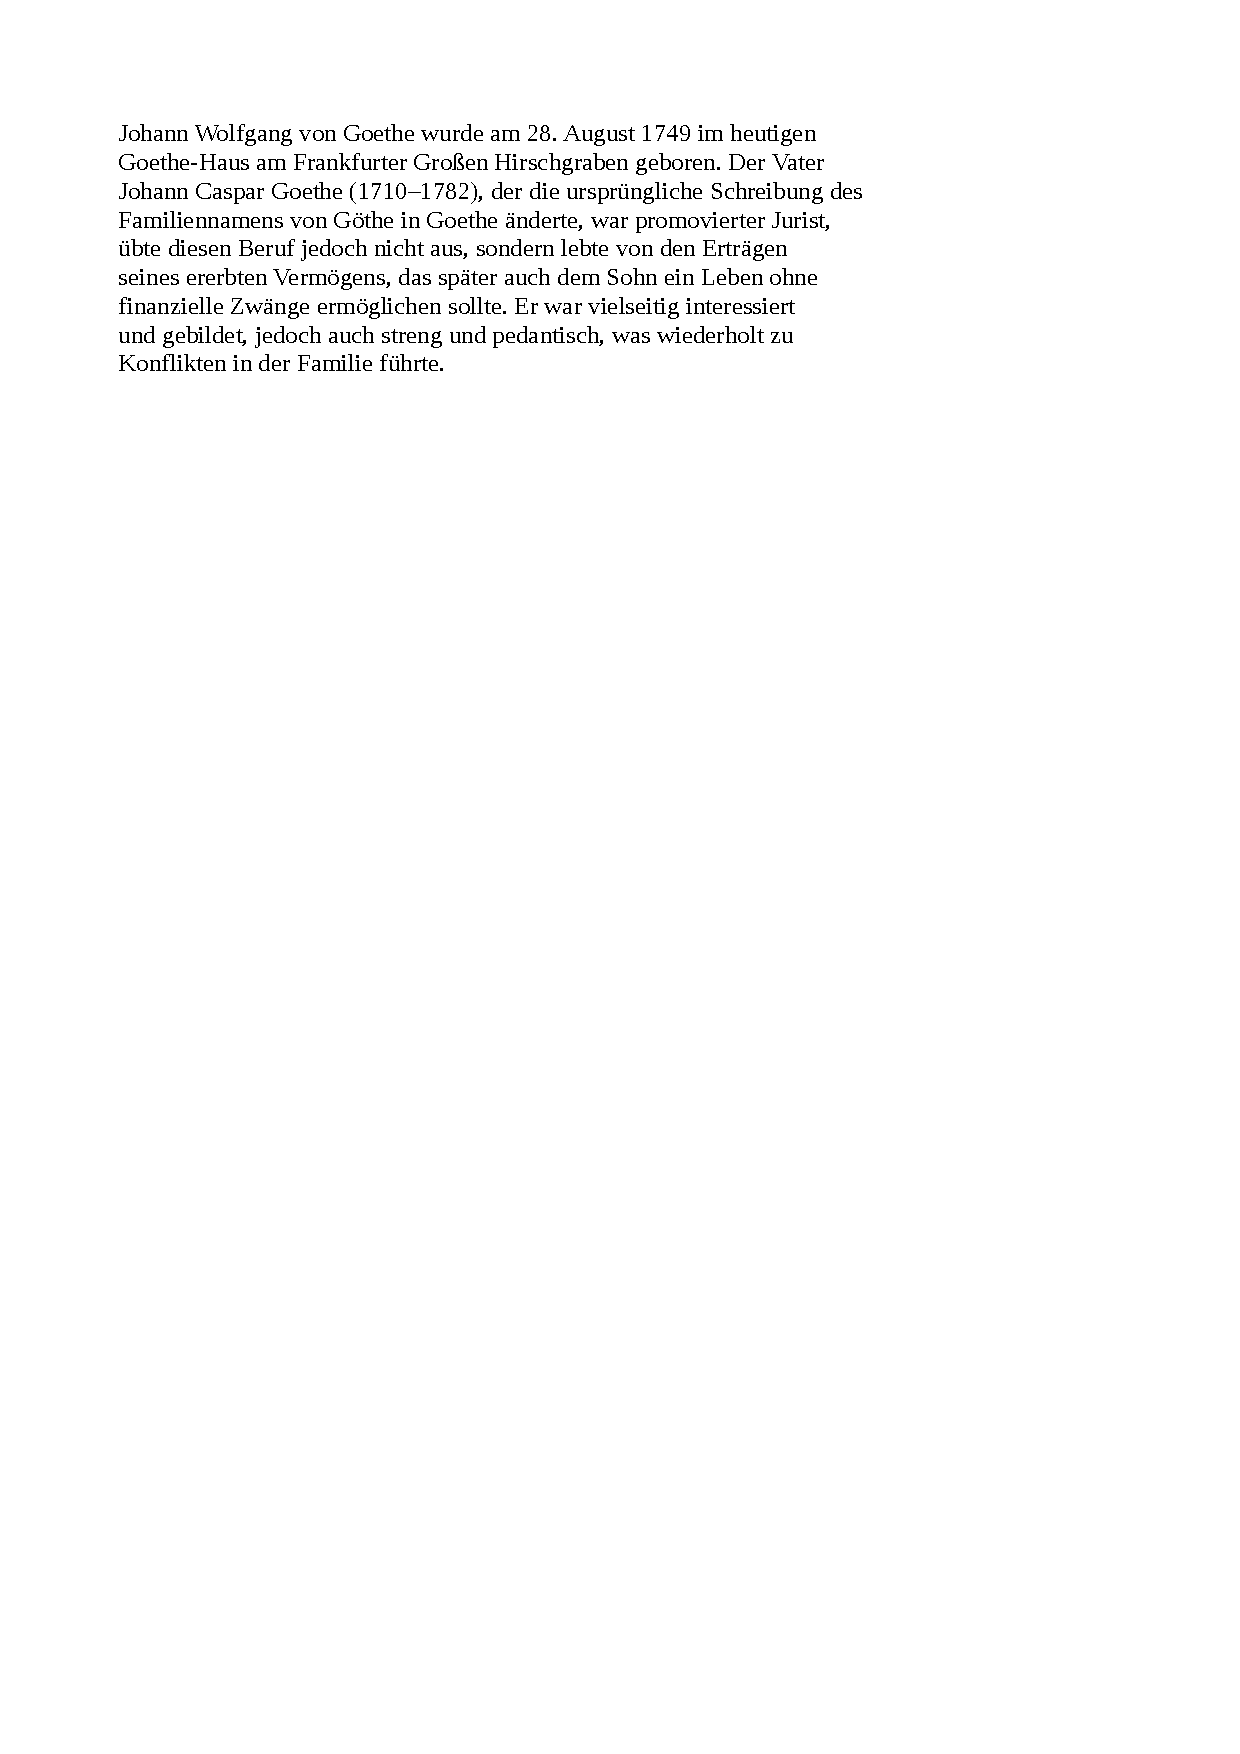
\includegraphics[scale=0.7]{Goethe.pdf}}
\end{picture}





%\begin{picture}(220,450)
%\put(40,80){ 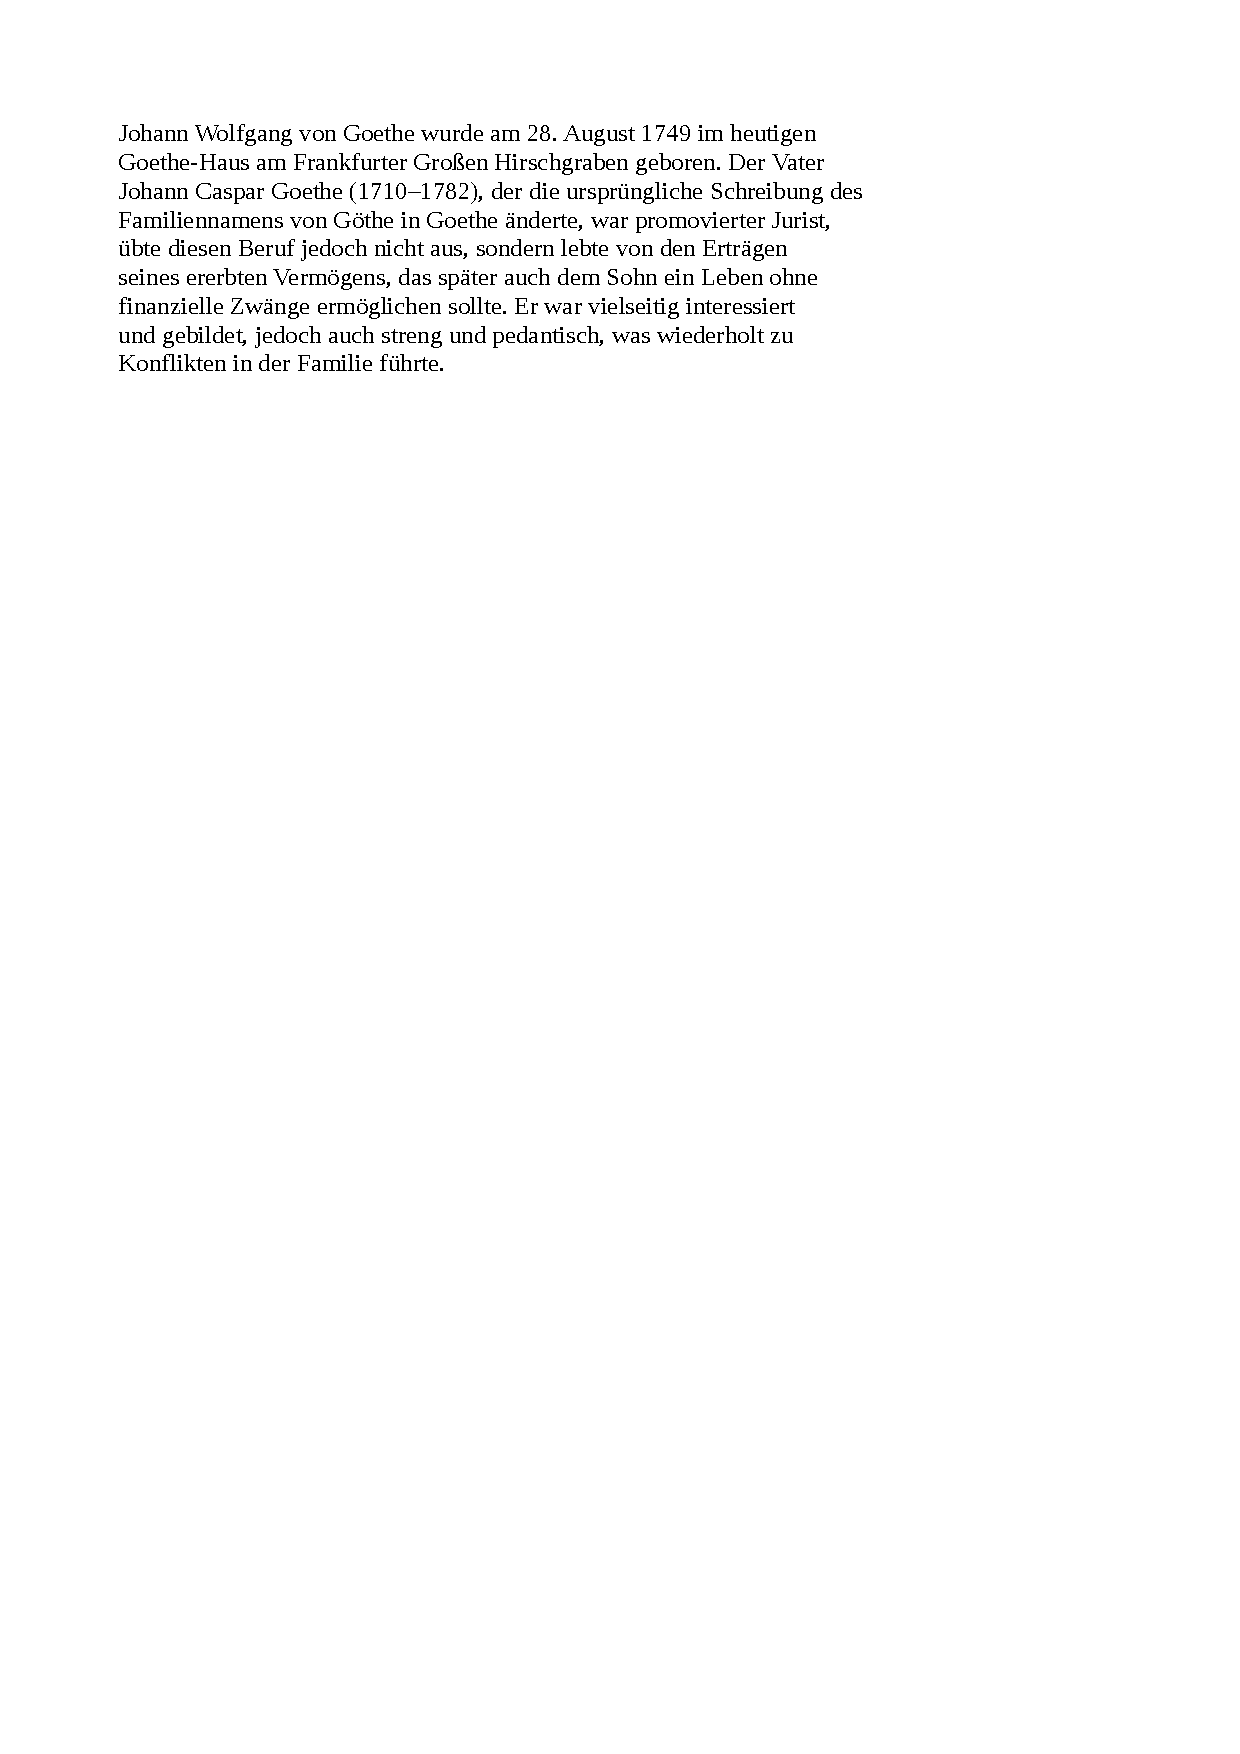
\includegraphics[height=15\textheight]{Goethe.pdf} }
%\end{picture}



\end{frame}


\begin{frame}
\frametitle{Wrong Hyphenation}
\begin{itemize}
\item Returns a list of all possible variations of a given text by hyphenating the last word.
\item Previous words are hyphenated through the execution of a Line Break operation.
\item For every line, find the last word and split it between the current and next line n-1 times, where n is the length of the word. 
\item Each division adds a new text to the list it returns, so there's a maximun of one new hyphenation per text in the list.
\item This way every possible combination is added to the list.
\item If a world is already hyphenated in a given line nothing is done at that line.
\end{itemize}
\end{frame}

\begin{frame}
\frametitle{Ensure Constraints}
\begin{itemize}
\item Our other operations are not concerned with keeping the text correct
\item This operation ensures that all constraints are met
\item In order to do this the algorithm goes from top to bottom
\item Shifting characters between the line being analyzed and the next line
	
\end{itemize}	
\end{frame}

\begin{frame}
\frametitle{Word Insertion}
\begin{picture}(0,190)
\put(30,0){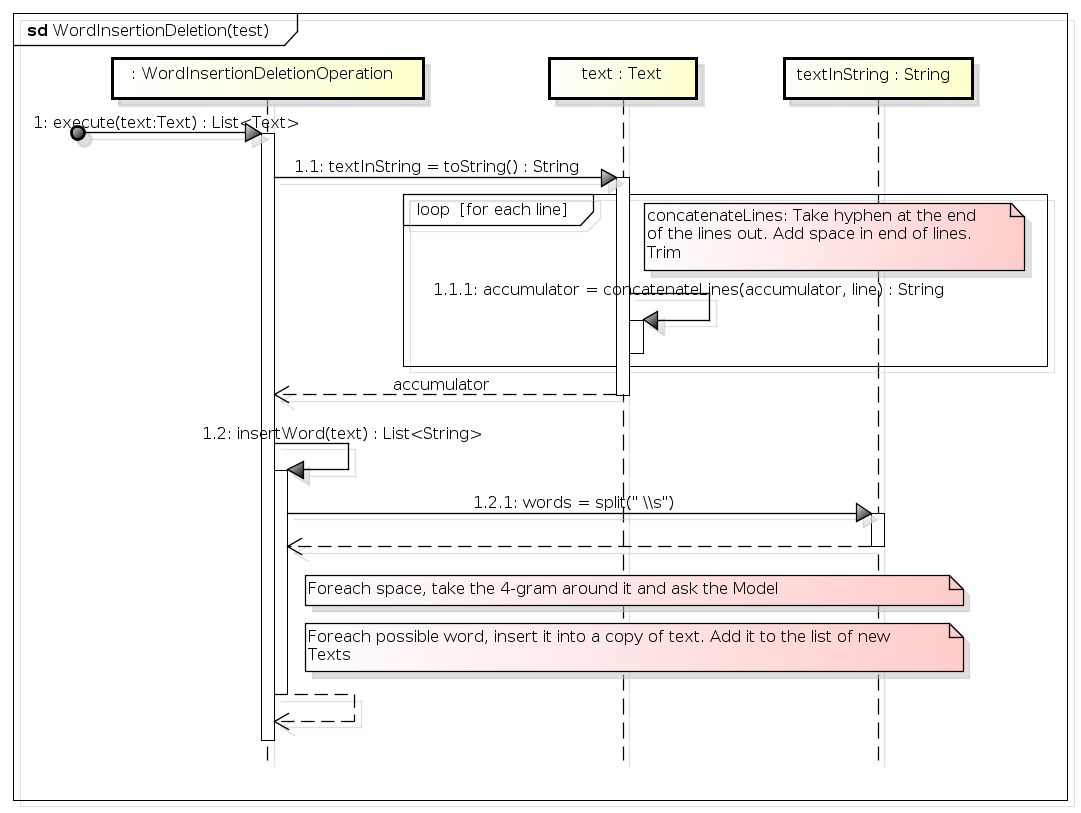
\includegraphics[scale=0.32]{img/WordInsertionDeletion.png}}
\end{picture}
\end{frame}

\begin{frame}
\frametitle{Word Insertion $-$ Databases}
\begin{itemize}
\item Current: Netspeak Requests  \emph{(netspeak.org)} \cite{Netspeak}
\item Possibility: Google NGram Database Manually Handled
\end{itemize}
\end{frame}

%------------------------------------------------
\section{First Results}
%------------------------------------------------

\begin{frame}
\frametitle{First Results $-$ Donald Knuth}
\texttt{\tiny Knuth ist der Sohn eines Lehrers. Er besuchte die Milwaukee Lutheran \\
High School und begann sein Physikstudium am California Institute of \\
Technology im September 1956. Aus zweierlei Gründen schlug er \\
tatsächlich seinem zweiten Studienjahr jedoch den Weg zur Mathematik \\
ein: Zum einen löste er ein Problem eines seiner \\
Mathematikprofessoren, was ihm eine 1,0 als Note einbrachte, zum \\
anderen fand er wenig Gefallen an den physikalischen Praktika. Er \\
erhielt einen Bachelor- und einen Master-Abschluss 1960 an der Case \\
Western Reserve University. 1963 erhielt er seinen Ph.D. vom \\
California Institute of Technology bei Marshall Hall, wo er dann auch \\
nach der Promotion Assistant Professor und 1966 Associate Professor \\
und schließlich Professor wurde. 1968 wurde er Professor für \\
Informatik an der Stanford University.\\}

Result Text: \\

\texttt{\scriptsize{K}\tiny nuth ist der Sohn eines Lehrers. Er besuchte die Milwaukee Luthera- \hskip 18pt \emph{//Wrong Hyphenation} \\
\scriptsize{n}\tiny  High School und begann sein Physikstudium am California Instit- \hskip 33pt \emph{//Line Break +} \\
\scriptsize{u}\tiny te of Technology im September 1956. Aus zweierlei Gründen schlug er \hskip 23pt \emph{//Wrong Hyphenation} \\
\scriptsize{t}\tiny atsächlich seinem zweiten Studienjahr jedoch den Weg zur Mat- \hskip 39pt \emph{//Wrong Hyphenation} \\
\scriptsize{h}\tiny ematik ein: Zum einen löste er ein Problem eines seiner \\
Mathematikprofessoren, was ihm eine 1,0 als Note einbrachte, zum \\
anderen fand er wenig Gefallen an den physikalischen Praktika. Er \\
erhielt einen Bachelor- und einen Master-Abschluss 1960 an der Case \\
Western Reserve University. 1963 erhielt er seinen Ph.D. vom \\
California Institute of Technology bei Marshall Hall, wo er dann auch \\
nach der Promotion Assistant Professor und 1966 Associate Professor \\
und schließlich Professor wurde. 1968 wurde er Professor für \\
Informatik an der Stanford University. \\}
\end{frame}

\begin{frame}
\frametitle{First Results $-$ Goethe}
\texttt{\tiny
Johann Wolfgang von Goethe wurde am 28. August 1749 im heutigen \\
Goethe-Haus am Frankfurter Großen Hirschgraben geboren. Der Vater \\
Johann Caspar Goethe (1710–1782), der die ursprüngliche Schreibung des \\
Familiennamens von Göthe in Goethe änderte, war promovierter Jurist, \\
übte diesen Beruf jedoch nicht aus, sondern lebte von den Erträgen \\
seines ererbten Vermögens, das später auch dem Sohn ein Leben ohne \\
finanzielle Zwänge ermöglichen sollte. Er war vielseitig interessiert \\
und gebildet, jedoch auch streng und pedantisch, was wiederholt zu \\
Konflikten in der Familie führte. \\
}

Result Text: \\

\texttt{\scriptsize{J}\tiny ohann Wolfgang von Goethe wurde am 28. August 1749 im he- \hskip 16pt \emph{//Wrong Hyphenation} \\
\scriptsize{u}\tiny tigen Goethe-Haus am Frankfurter Großen Hirschgraben gebore- \hskip 10pt \emph{//LineBreak + Wrong Hyphenation} \\
\scriptsize{n}\tiny . Der Vater Johann Caspar Goethe (1710–1782), der die ursprün- \emph{//Wrong Hyphenation} \\
\scriptsize{g}\tiny liche Schreibung des Familiennamens von Göthe in Goethe änderte, war \\
promovierter Jurist, übte diesen Beruf jedoch nicht aus, sondern lebte \\
von den Erträgen seines ererbten Vermögens, das später auch dem Sohn \\
ein Leben ohne finanzielle Zwänge ermöglichen sollte. Er war \\
vielseitig interessiert und gebildet, jedoch auch streng und \\
pedantisch, was wiederholt zu Konflikten in der Familie führte. \\
}
\end{frame}

\begin{frame}
\frametitle{First Results $-$ Berlin}

\texttt{\tiny
Berlin ist die Hauptstadt und zugleich ein Land der Bundesrepublik \\
Deutschland. Der Stadtstaat Berlin bildet eine Einheitsgemeinde und \\
ist mit über 3,4 Millionen Einwohnern die bevölkerungsreichste und mit \\
knapp 892 Quadratkilometern die flächengrößte Kommune Deutschlands \\
sowie nach Einwohnern die zweitgrößte der Europäischen Union. Zudem \\
ist Berlin mit rund 3800 Einwohnern je Quadratkilometer die am \\
drittdichtesten bevölkerte Gemeinde Deutschlands. Berlin ist eine \\
Enklave im Land Brandenburg und bildet das Zentrum der Metropolregion \\
Berlin/Brandenburg (6 Millionen Einwohner) sowie der Agglomeration \\
Berlin (4,4 Millionen Einwohner). Der Stadtstaat unterteilt sich in \\
zwölf Bezirke. \\
}

Result Text: \\

\texttt{\scriptsize{B}\tiny erlin ist die Hauptstadt und zugleich ein Land der Bundesrepubl- \hskip 15pt \emph{//Wrong Hyphenation} \\
\scriptsize{i}\tiny k Deutschland. Der Stadtstaat Berlin bildet eine \hskip 62pt \emph{//Line Break + Line Break} \\
\scriptsize{E}\tiny inheitsgemeinde und ist mit über 3,4 Millionen Einwohne- \hskip 40pt \emph{//Wrong Hyphenation} \\
\scriptsize{r}\tiny n die bevölkerungsreichste und mit knapp 892 Quadratkilometern die \\
flächengrößte Kommune Deutschlands sowie nach Einwohnern die \\
zweitgrößte der Europäischen Union. Zudem ist Berlin mit rund 3800 \\
Einwohnern je Quadratkilometer die am drittdichtesten bevölkerte \\
Gemeinde Deutschlands. Berlin ist eine Enklave im Land Brandenburg und \\
bildet das Zentrum der Metropolregion Berlin/Brandenburg (6 Millionen \\
Einwohner) sowie der Agglomeration Berlin (4,4 Millionen Einwohner). \\
Der Stadtstaat unterteilt sich in zwölf Bezirke. \\
}
\end{frame}

%------------------------------------------------
\section{Next Steps}
%------------------------------------------------

\begin{frame}
\frametitle{Next Steps}
\begin{itemize}
\item 
\item 
\item 
\item 
\end{itemize}
\end{frame}

%------------------------------------------------
\section{References}
%------------------------------------------------

\begin{frame}
\frametitle{References}
\footnotesize
\begin{thebibliography}{1}
\bibitem{Stein}
	Benno Stein, Matthias Hagen, and Christof Bräutigam. \emph{Generating Acrostics via Paraphrasing and Heuristic Search}. \\
	In Junichi Tsujii and Jan Hajic, editors, 25th International Conference on Computational Linguistics (COLING 14), pages 2018-2029, August 2014. Association for Computational Linguistics. 
\bibitem{Netspeak}
	Martin Potthast, Martin Trenkmann, and Benno Stein.
	\emph{Netspeak: Assisting Writers in Choosing Words}. \\
	In Cathal Gurrin et al, editors, Advances in Information Retrieval. 32nd European Conference on Information Retrieval (ECIR 10) volume 5993 of Lecture Notes in Computer Science, pages 672, Berlin Heidelberg New York, March 2010. Springer.
\end{thebibliography}
\end{frame}
%------------------------------------------------

\begin{frame}
\Huge{\centerline{Questions?}}
\end{frame}

%----------------------------------------------------------------------------------------

\end{document}
